\documentclass[2126824.tex]{subfiles}

\begin{document}
Following the discovery and destruction of a Vespa mandarinia hornet nest there have been multiple sightings of this largest wasp in the world. Even at small numbers they are capable of destroying colonies of bees at brutal efficiency, so it is crucial that the spread of these wasps is curbed and eradicated.

The data-set that we are given to work with has a bunch of useful and interesting variables off which we can base our models. Latitude/Longitude is most obvious with potential for a geospatial analysis, the inclusion of pictures allowed us to look into possibly developing a neural network to identify the wasp based on the picture, and most interestingly the notes included allowed us to set up a frequency analysis model and see if the included notes columns can be used to determine whether the observation had the wasp in it or not.

\subsection{Introductory Visual Analysis}

Looking at an overview of the situation, we can pinpoint exactly where we can focus on for the overall spread of the wasp.

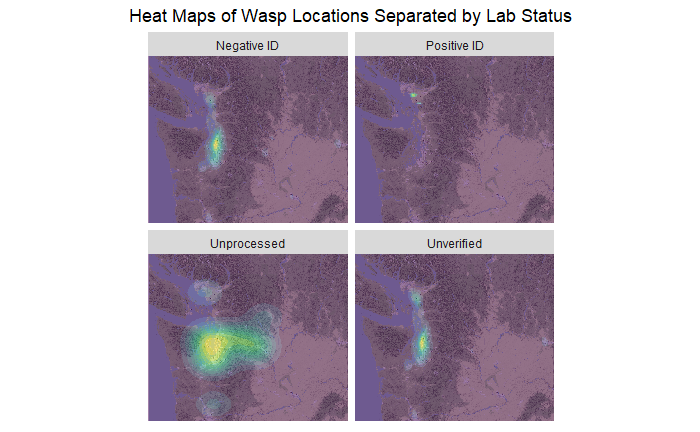
\includegraphics[width=\textwidth]{name/facet_full.png}

It can be seen that all the current confirmed cases are in the North Western part of Washington so we can fairly safely zoom in and look at that specific region. 



\end{document}